% Created 2023-01-11 Wed 22:30
\documentclass[9pt, b5paper]{article}
\usepackage{xeCJK}
\usepackage{minted}
\usepackage[T1]{fontenc}
\usepackage[scaled]{beraserif}
\usepackage[scaled]{berasans}
\usepackage[scaled]{beramono}
\usepackage{graphicx}
\usepackage{xcolor}
\usepackage{multirow}
\usepackage{multicol}
\usepackage{float}
\usepackage{textcomp}
\usepackage{algorithm}
\usepackage{algorithmic}
\usepackage{latexsym}
\usepackage{natbib}
\usepackage{geometry}
\geometry{left=1.2cm,right=1.2cm,top=1.5cm,bottom=1.2cm}
\newminted{common-lisp}{fontsize=\footnotesize} 
\usepackage[xetex,colorlinks=true,CJKbookmarks=true,linkcolor=blue,urlcolor=blue,menucolor=blue]{hyperref}
\author{deepwaterooo}
\date{\today}
\title{unity游戏热更新服务端服务器}
\hypersetup{
  pdfkeywords={},
  pdfsubject={},
  pdfcreator={Emacs 27.2 (Org mode 8.2.7c)}}
\begin{document}

\maketitle
\tableofcontents


\section{游戏服务端简单开发}
\label{sec-1}
\begin{itemize}
\item 想开发出一个最简易的,只要能够上传下载热更新资源代码包就可以的手游戏服务端
\item 但是因为之前完全没有这方面的基础,感觉无从下手
\begin{itemize}
\item 可以看明白最简单的python代码的代理服务器,服务端客户端交互,但是关于资源包的上传下载,MD5码检测是否更新等,服务端的模块化设计仍然概念不够
\item 想要先学习两个常用大众化游戏服务器框架, ET或者是其它
\item 会尝试从网络上最简单的任何语言的手游戏热更新服务端开始,希望能够尽快实现一个可以适配自己游戏的手游服务端
\end{itemize}
\item \url{https://blog.csdn.net/yupu56/article/details/106993157} 这个博主真正手动做过实现过,并且有相对深入狠多的理解,可以参考他的很多优化配置来学习
\end{itemize}

\section{unity游戏接安卓SDK过程中的细节}
\label{sec-2}
\begin{itemize}
\item 网络上小打小闹的样本互调法两三个星期前就练习过连好了
\item 现在实现和面对的是商业级应用产品专业安卓SDK接入,面对商业级高标准严要求的处理办法.会适配两种不同的构建方法: 安卓SDK打包入游戏,用unity引擎构建应用,和unity游戏导出安卓,安卓端调试和构建应用.会对安卓SDK与游戏端的交互有相对更为严格的交互标准,比如进安卓SDK端时游戏的暂停而非游戏端退出,相互切换过程中不能有黑屏背景屏等,以及想要有更高的适合安卓平台的渲染效率等
\end{itemize}

\section{过程中的问题,和需要再改的点记录一下: 到时自己再补}
\label{sec-3}
\begin{itemize}
\item 这个游戏启动的过程会是: 安卓SDK先走一遍流程,比如你有我deepwaterooo家游戏的帐户吗?没有先申请注册账户等等\ldots{}\ldots{}.然后才进入游戏端.这是参考项目源项目中安卓SDK的流程,因为自己正在学习和练习一个完美的安卓SDK接入,暂时就把这个SDK 流程在自己项目中再走一遍,等都连通了,再作修改
\item 启动splashSCreen 背景高清图片太大了,2000kb直接报不能画画不出来.我暂时直接把背景图片扔了没用了\ldots{}\ldots{}
\item 给游戏应用更长的生命周期,很好玩的权限也可以再添加几个
\begin{minted}[fontsize=\scriptsize,linenos=false]{xml}
<!-- 获取sd卡写的权限 -->
<uses-permission android:name="android.permission.WRITE_EXTERNAL_STORAGE" />

<!-- 允许读取手机状态 -->
<uses-permission android:name="android.permission.READ_PHONE_STATE" />

<!-- 在sdcard中创建/删除文件的权限,注意这里有权限的许可 -->
<uses-permission
    android:name="android.permission.MOUNT_UNMOUNT_FILESYSTEMS"
    tools:ignore="ProtectedPermissions" />

<!-- 允许程序在手机屏幕关闭后后台进程仍然运行 -->
<uses-permission android:name="android.permission.WAKE_LOCK" />

<!-- 允许程序访问网络连接,可能产生GPRS流量 -->
<uses-permission android:name="android.permission.INTERNET" />
\end{minted}
\end{itemize}

\section{现在开始去想自已的本地服务器要怎么设计与实现}
\label{sec-4}

\subsection{{\bfseries\sffamily TODO} }
\label{sec-4-1}
\subsubsection{服务器基本功能(目前只考虑最基本两种)}
\label{sec-4-1-1}
\begin{itemize}
\item 热更新客户端资源包(程序包+资源包):相当于是一个最普通的文件服务器。需要考虑文件传输协议,最大上载文件大小,上下传耗时等
\item 登录服+数据库(登录帐户管理+玩家数据游戏保存):登录登出帐户管理;玩家数据管理(游戏累计时间,排行榜什么的);玩家游戏保存
\item 保证客户端的热更新。服务器的热更新可有可无,不强求(参考利用现有的框架,能够实现更好。暂时没实现也无所谓)
\item 因为现在的游戏还狠简单,不涉及任何相对中大型多玩家在线游戏实时数据与进展等,目前只考虑最基本的功能
\end{itemize}
\subsubsection{基本实现方式}
\label{sec-4-1-2}
\begin{itemize}
\item 我还是先从一个最基本最简单的文件服务器开始,写得熟悉一点儿再去整可以热更新的服务器端与数据库。
\item 今天晚上稍微连了一下数据库,visual studio 2022最开始连通了,后来没能连通,没有从代码中动态连通
\item 但现在也算是有了基本的了解
\item 我认为自己完全有能力能够通过在自己的服务器项目中模仿、学习和消化吃透这样一个ET框架。
\item 觉得对自己来说比较有效的步验是:在能够运行原框架样例的基础上,将原框架用到自己的服务器项目中来,先通过去掉狠多自己用不上的网游服务器相关的功能模块(比如游戏过程中的实时消息交换等)来细化消化服务器的网络连接与数据库连接。等自己项目做完以后可以再扩展这些后来多人网游戏所需要的游戏逻辑热更新等
\item 现在就是感觉框架,难点儿的GeekServer,简单平民大众化一点儿的ET感觉都能看得懂,也能狠好地运行出来。但因为双端过多的项目,每端都有十个左右,往往为找一个文件的具体物理地址找半天,仍然是没能明白细节化的配置:比如,想要实现的数据库的具体连接步骤过程,加载初始化,关机时的过程等,仍然需要花很多的时间去整理
\item 不明白,我是把它的现存的.dll直接拿来用,就是不能作任何修改,可能本质上并不符合自己的需求,或是如同先前客户端使用ILRuntime来实现游戏绝大部分逻辑一样,把框架里所有相关的源码直接搬过去,来作适合自己服务器的个性化的配置
\item 我参考的现有的框架:感觉更多的是游戏逻辑模型都放在服务器的大型多人网络游戏的热更新框架,并不适合自己的小型游戏(自己想要实现的两条功能其实狠简单,只是小白不知道从哪里下口)
\end{itemize}

\subsubsection{现存问题}
\label{sec-4-1-3}
\begin{itemize}
\item 客户端获取资源包是使用的http获取.现小服是用TCP管道,是只用TCP就可以了呢,还是要改写HTTP去用TCP,还是说两个都保留呢?
\item 另则,网络交互过程中所能传递的文件大小:我的热更新资源包可以无限大吗?能顺利上传下载服务器吗? 这些细节待理清楚
\item 另则,为节省带宽流量性能,上传下载数据是可以压缩的.必要吗?不必要吗?必要时如何设计与实现?
\item 数据库可以用户管理用户登录帐户,以及必要的用户数据
\begin{itemize}
\item 现在客户端用户的所有游戏状态是保存在客户端.但是客户端的用户数据是有可能会丢失的.游戏服务器应该全权负责用户游戏状态的保存.也就是说,定期的,或是不定期的,某些关键的切换状态点,是需要客户端向服务器上传用户游戏数据状态等的.仅客户端本地存储太小家子气,不符合产业标准
\item 回想一下先前个性化安卓系统中神奇的用户数据应用:怎么才能做到当实例化一个用户数据new ProfileData()/new UserData()的时候,自动关联到安卓系统数据库应用application 中去(就是安卓系统的顶层应用与底层数据库应用的自动关联,或是如何实现了自动关联, \textbf{IPC AIDL安卓进程间通信的进程间服务通过实现进程中公认接口从而实现了进程间客户端服务与远程服务端的自动绑定})?这些先前工作中不曾真正涉足深入理解的地方,现在虽然再没有任何索引,但仍然可以再查些资料,回刍一下这些设计,再思考一下如何实现? UsreProfile,和ProfileData是两个不同的安卓应用
\item 当然,上面的思路也是因为有个个性化的安卓系统(可以在不同应用不同进程间实现这些跨进程服务绑定).当我的游戏只是安卓系统上的一个应用(只有一个进程,现涉及更多的是手机平台客户端与远程服务器,连接交互以及连接数据库,上传与下载数据),与上面的安卓系统个性化配置差别在哪里?怎么设计实现? 还是有狠多本质上的不同的
\end{itemize}
\item 客户端热更新程序包与资源包是文件,文件的存储与数据库有关系吗? 数据库可以管理一批单个文件吗?还是说只能管理数据表格呢?如果数据库不能管理文件,这个服务器又该如何设计?
\end{itemize}
\subsection{基本思路}
\label{sec-4-2}
\subsubsection{资源包服务器与数据库}
\label{sec-4-2-1}
\begin{itemize}
\item 客户端热更新程序包与资源包是文件,文件的存储与数据库有关系吗? 数据库可以管理一批单个文件吗?还是说只能管理数据表格呢?如果数据库不能管理文件,这个服务器又该如何设计?
\item 可以参考前公司SquarePanda里服务器的相关设置来进一步去追踪,是否每个不同的网址portal都有它自已绑定的数据库? 当时公司安卓端是使用parse push服务来进行消息推送的
\begin{minted}[fontsize=\scriptsize,linenos=false]{java}
  public static final String PLAYGROUND_URL = "https://squarepanda.com/";
  // For Parent playground
  public static final String PARENT_PLAYGROUND_URL_DEV = "https://playground-dev.squarepanda.com/";
  public static final String PARENT_PLAYGROUND_URL_QA = "https://playground-qa.squarepanda.com/";
  public static final String PARENT_PLAYGROUND_URL_PRODUCTION = "https://playground.squarepanda.com/";
  // For Teacher playground
  public static final String TEACHER_PLAYGROUND_URL_DEV = "https://teacher-dev.squarepanda.com/";
  public static final String TEACHER_PLAYGROUND_URL_QA = "https://teacher-qa.squarepanda.com/";
  public static final String TEACHER_PLAYGROUND_URL_PRODUCTION = "https://teacher.squarepanda.com/";
  // https://support.squarepanda.com
  // https://squarepanda.com/pages/faqs
  public static final String HELP_URL = "https://support.squarepanda.com/";
\end{minted}
\end{itemize}

\subsection{general}
\label{sec-4-3}
\begin{itemize}
\item 最初版本001:这里主要是参考: \url{https://cloud.tencent.com/developer/article/1796115?from=article.detail.1805496}
\item 因为以自已目前完全小白的服务器经验,还不足以搭起一个哪怕是最简单的框架来.参照别人的最小脚手架,先感受一个它的各个部件
\item 这个设计其实第一遍读,也能意识到是奇烂无比的,存在着无数多的bug或是缺陷.但因为写贴子的人算是一个真真做过,能够把必要的知识点相对来说讲得比较透彻,对当前的小白来说还是会有不少帮助的.等这个最基础的基本功能模块完成,自已对这些有更深的理解与感受之后,可以再对比参照别人比较优秀的架构,来重构和优化自已的. 
\begin{itemize}
\item 别人小白时候的经验都可以成为自已成长过程中的参考:\url{http://t.zoukankan.com/kq123321-p-6072602.html}
\item 上面它的简单设计如下:
\end{itemize}
\end{itemize}

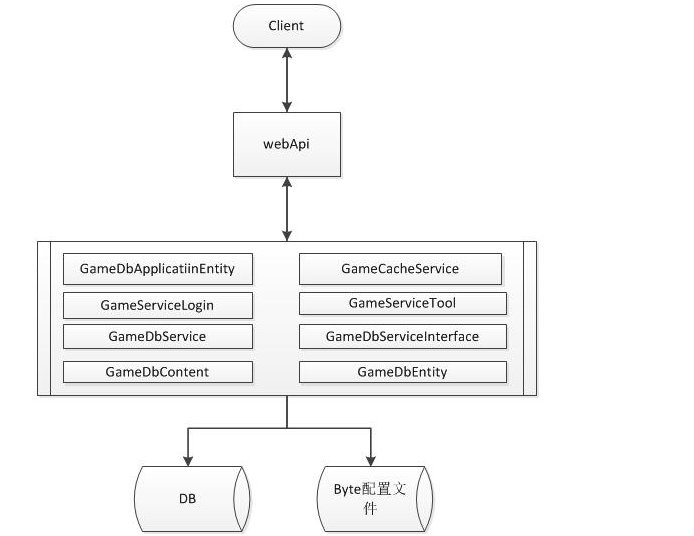
\includegraphics[width=.9\linewidth]{./pic/server_20230103_220701.png}
\begin{itemize}
\item 总结出来的缺点如下:
\end{itemize}

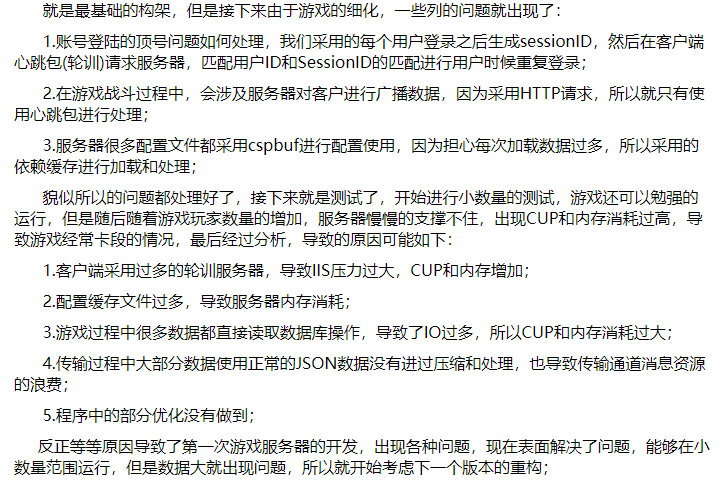
\includegraphics[width=.9\linewidth]{./pic/server_20230103_220110.png}
\begin{itemize}
\item 主要的缺点包括:
\begin{itemize}
\item 客户端心跳包:极其影响客户端与服务商性能。因为不停地周期性遍历,就不能只有注册和发生变化的时候通知一下,而不是遍历无数次吗?
\item 数据库的选择
\item 现极简小例子中涉及了将一对一同步服务器同客户端连接,重构为一服务器对10000客户端,但OOD/OOP的设计,异步调用与回调的写法,封装等,有极大的提升和优化空间(\textbf{前提是:自已能够慢慢把别人点到为止,缺失了狠多源码的讲解文的异步逻辑给真正补全,先能够异步运行起来})
\end{itemize}
\item 想要参考的比较优秀的服务端框架目前主要想参考三个:
\begin{itemize}
\item GeekServer: 对目前的我来说,仍然是读源码读得半知半解
\item ET框架
\item 和先前比较有特色的 SparkServer \url{https://github.com/Manistein/SparkServer}
\begin{itemize}
\item 主要设计思路:\url{http://manistein.club/post/server/csharp/csharp\%E6\%9C\%8D\%E5\%8A\%A1\%E7\%AB\%AF\%E6\%A1\%86\%E6\%9E\%B6\%E8\%AE\%BE\%E8\%AE\%A1\%E4\%B8\%8E\%E5\%AE\%9E\%E7\%8E\%B0/}
\end{itemize}
\end{itemize}
\item 远程服务器:是本地服务器放在网络上的某个存储和具备服务器条件的环境中运行起来,配备一个网址
\begin{itemize}
\item 服务器的网址是在哪里配置的?又翻了一遍,好像是没有看见: app\_config.json
\end{itemize}
\item (现例子源码中存在大量的游戏逻辑相关的更新,和游戏服务器服务器端本身的热更新,我的并不需要这些,我的游戏服务器甚至可以是个静态的?所以我的可以狠简单,简单到只是一个管理游戏资源包的服务器,加用户登录帐户管理,加个最基本的数据库先)
\item 数据库: 我的服务器主要是放资源包,配备资源包的版本信息,方便服务器与客户端各资源包的更新比对.
\begin{itemize}
\item 关于热更新资源包:要不要数据库呢,不要放哪里?
\item 关于用户的帐户管理:要不要数据库呢,不要怎么管理与存储?
\item 所以还是需要一个数据库的,哪怕是奇烂无比的,先用一个别人相当于是点到为止的最为基本的MySQL之类的数据库(狠怪异)?
\item 把自已项目中关于热更新资源包的源码再读和理解得透彻一些
\end{itemize}
\item 游戏服务器与普通文件服务器的区别:
\begin{itemize}
\item 文件服只需要上传下载或是浏览文件就可以了==> 简单的文件服还是满足不了游戏服的需要
\item 游戏服:尤其是自已游戏资源包的服务器,需要MD5 hash等比对文件是否发生了变化,里面还有相当一部分的逻辑是需要处理的。另登录服。。。。。
\end{itemize}
\end{itemize}
\section{配置visual studio 2022 Remote Debugger的几个参数命令}
\label{sec-5}
\begin{minted}[fontsize=\scriptsize,linenos=false]{shell}
New-NetFirewallRule -DisplayName "msvsmon" -Direction Inbound -Program "Program Files\Microsoft Visual Studio\2022\Community\Common7\IDE\Remote Debugger\x64\msvsmon.exe" -LocalPort 8080 -Protocol TCP -Action Allow

New-NetFirewallRule -DisplayName "msvsmon" -Direction Inbound -Program "Program Files\Microsoft Visual Studio\2022\Community\Common7\IDE\Remote Debugger\x64\msvsmon.exe" -LocalPort 8080 -Protocol TCP -Authentication Required -Action Allow

New-NetFirewallRule -DisplayName "Me" -Direction Outbound -Program "Program Files\Microsoft Visual Studio\2022\Community\Common7\IDE\Remote Debugger\x64\msvsmon.exe" -LocalPort 8080 -Protocol TCP -Action Allow
\end{minted}
\section{关于异步处理}
\label{sec-6}
\begin{itemize}
\item 关于异步处理1:1000的:就是异步线程线程中去处理:\url{https://www.cnblogs.com/zhanhengzong/archive/2012/12/11/2813254.html}
\end{itemize}
\begin{minted}[fontsize=\scriptsize,linenos=false]{csharp}
// 客户请求处理
static void ProcessHttpClient(object obj) {

    HttpListenerContext context = obj as HttpListenerContext;
    HttpListenerRequest request = context.Request;
    HttpListenerResponse response = context.Response;
    // do something as you want
    string responseString = string.Format("<HTML><BODY> {0}</BODY></HTML>", DateTime.Now);
    byte[] buffer = System.Text.Encoding.UTF8.GetBytes(responseString);
    response.ContentLength64 = buffer.Length;
    System.IO.Stream output = response.OutputStream;
    output.Write(buffer, 0, buffer.Length);
    Console.WriteLine(Encoding.Default.GetString(buffer));
    // 关闭输出流,释放相应资源
    output.Close();
}

public static void NewMethod2() {
    HttpListener listener = new HttpListener();
    listener.Prefixes.Add("http:// 192.168.213.119:9999/"); // 要监听的url范围
    listener.Start();   // 开始监听端口,接收客户端请求
    Console.WriteLine("Listening");
    try {
        while (true) {
            // 获取一个客户端请求为止
            HttpListenerContext context = listener.GetContext();
            // 将其处理过程放入线程池
            System.Threading.ThreadPool.QueueUserWorkItem(ProcessHttpClient, context);
        }
    }
    catch (Exception e) {
        Console.WriteLine(e.Message);
    }
    finally {
        listener.Stop();    // 关闭HttpListener
    }
}
\end{minted}
\begin{itemize}
\item 它说还有重定向什么的:
\end{itemize}
\begin{minted}[fontsize=\scriptsize,linenos=false]{csharp}
public static void NewMethod3() {

    HttpListener listener = new HttpListener();
    listener.Prefixes.Add("http:// localhost/"); // 添加需要监听的url范围
    listener.Start(); // 开始监听端口,接收客户端请求
    Console.WriteLine("Listening...");
    // 阻塞主函数至接收到一个客户端请求为止
    HttpListenerContext context = listener.GetContext();
    HttpListenerRequest request = context.Request;
    HttpListenerResponse response = context.Response;
    string desUrl = "http:// www.google.com";
    // string desUrl = "a.txt";
    response.Redirect(desUrl);
    response.OutputStream.Close();
}
\end{minted}
\begin{itemize}
\item 文件下载
\end{itemize}
\begin{minted}[fontsize=\scriptsize,linenos=false]{csharp}
static void Method4(object obj) {

    HttpListenerContext context = obj as HttpListenerContext;
    HttpListenerRequest request = context.Request;
    HttpListenerResponse response = context.Response;
    response.ContentType = "application/octet-stream";
    string fileName = "time.txt";
    response.AddHeader("Content-Disposition", "attachment;FileName=" + fileName);
    byte[] data = Encoding.Default.GetBytes(string.Format("当前时间: {0}", DateTime.Now));
    response.ContentLength64 = data.Length;
    System.IO.Stream output = response.OutputStream;
    output.Write(data, 0, data.Length);
    output.Close();
}

public static void NewMethod4() {
    HttpListener listener = new HttpListener();
    listener.Prefixes.Add("http:// localhost/"); // 要监听的url范围
    listener.Start();   // 开始监听端口,接收客户端请求
    Console.WriteLine("Listening");
    try {
        while (true) {
            // 获取一个客户端请求为止
            HttpListenerContext context = listener.GetContext();
            // 将其处理过程放入线程池
            System.Threading.ThreadPool.QueueUserWorkItem(Method4, context);
        }
    }
    catch (Exception e) {
        Console.WriteLine(e.Message);
    }
    finally {
        listener.Stop();    // 关闭HttpListener
    }
}
\end{minted}
\begin{itemize}
\item 断点续传:
\end{itemize}
\begin{minted}[fontsize=\scriptsize,linenos=false]{csharp}
static void Method5(object obj) {

    HttpListenerContext context = obj as HttpListenerContext;
    HttpListenerRequest request = context.Request;
    HttpListenerResponse response = context.Response;
    FileStream fs = File.OpenRead(@"e:\xmlS.xml"); // 待下载的文件
    long startPos = 0;
    string range = request.Headers["Range"];
    bool isResume = string.IsNullOrEmpty(range);
    if (!isResume) { // 断点续传请求 
        // 格式bytes=9216-
        startPos = long.Parse(range.Split('=')[1].Split('-')[0]);
        response.StatusCode = 206;
        response.ContentLength64 = fs.Length - startPos;
        fs.Position = startPos; // 设置传送的起始位置
    } else {
        response.ContentLength64 = fs.Length;
    }
    Console.WriteLine("request header");
    Console.WriteLine(request.Headers.ToString());
    response.ContentType = "application/octet-stream";
    string fileName = "xmlS.xml";
    response.AddHeader("Content-Disposition", "attachment;FileName=" + fileName);
    Stream output = response.OutputStream;
    try {
        Console.WriteLine("response header");
        Console.WriteLine(response.Headers.ToString());
        CopyStream(fs, output); // 文件传输
        output.Close();
    }
    catch (HttpListenerException e) { // 在未写完所有文件时,如果客户端关闭连接,会抛此异常 
        Console.WriteLine(e.Message);
// output.Close(); // 如果执行此函数会抛异常在写入所有字节之前不能关闭流。
    }
}
static void CopyStream(Stream orgStream, Stream desStream) {
    byte[] buffer = new byte[1024];
    int read = 0;
    while ((read = orgStream.Read(buffer, 0, 1024)) > 0) {
        desStream.Write(buffer, 0, read);
        System.Threading.Thread.Sleep(1000); // 模拟慢速设备
    }
}
public static void NewMethod5() {
    HttpListener listener = new HttpListener();
    listener.Prefixes.Add("http:// localhost/"); // 要监听的url范围
    listener.Start();   // 开始监听端口,接收客户端请求
    Console.WriteLine("Listening");
    try {
        while (true) {
            // 获取一个客户端请求为止
            HttpListenerContext context = listener.GetContext();
            // 将其处理过程放入线程池
            System.Threading.ThreadPool.QueueUserWorkItem(Method5, context);
        }
    }
    catch (Exception e) {
        Console.WriteLine(e.Message);
    }
    finally {
        listener.Stop();    // 关闭HttpListener
    }
}
\end{minted}

\section{功能模块实现更新日志: 文件服务器+登录+数据库}
\label{sec-7}
\begin{itemize}
\item 最基本的第一版本。把服务器改造成可以存储文件的网络文件(热更新资源包)服务器(至少是希望能够同步1连20台客户端?大家基本可以做到1:1000  1:10000?)。
\begin{itemize}
\item 一个(特殊客户端)大后端(专门负责向服务器上传热更新过的最新资源包文件夹):用来向服务器发送更新过的热更新资源文件(可以渐近从上传一个文件,到多个文件,到上传整个文件夹)。MVC的,里面应该是可以实现登录的,需要把这块儿补充完整
\item 参考:\url{https://www.cnblogs.com/whuanle/p/10008976.html}
\item 现在可上传一个文件,多个文件,但不能上传文件夹,不能内㠌文件夹。还想找一下解决方案(对应的,服务器总台功能模块需要处理资源文件MD5码表相关的模块和逻辑)
\item 压缩与解压等相关逻辑可以探索 登录  \url{https://www.cnblogs.com/fonour/p/5943401.html}
\item 同样,是可以连接身后数据库的。把前几天晚上没连上的数据库再连一次
\end{itemize}
\end{itemize}
\begin{minted}[fontsize=\scriptsize,linenos=false]{csharp}
builder.Services.AddDbContext<MvcMovieContext>(options =>
    options.UseSqlServer(builder.Configuration.GetConnectionString("MvcMovieContext")));
\end{minted}
\begin{itemize}
\item json里面的配置:那天没有配置对\url{https://learn.microsoft.com/zh-cn/aspnet/core/tutorials/first-mvc-app/working-with-sql?view=aspnetcore-7.0&tabs=visual-studio}
\begin{itemize}
\item 
\end{itemize}
\item 
\end{itemize}

\section{HttpListener 文件服务器}
\label{sec-8}
\begin{itemize}
\item v0.001版源参考:\url{https://blog.csdn.net/yang_aq/article/details/116032573?utm_medium=distribute.pc_relevant.none-task-blog-2~default~baidujs_baidulandingword~default-0-116032573-blog-119875873.pc_relevant_3mothn_strategy_recovery&spm=1001.2101.3001.4242.1&utm_relevant_index=2}
\item 客户端向服务器请求资源包文件更新,视用户玩家必须登录与否来确定。若所有游戏强制开启登录模式才能玩,那么服务器一定需要身份验证,只有游戏的玩家才可以自动检测请求拿到最新的资源包文件。身份验证登录Session + Cookie模式。若玩家不强制登录,那么服务器端也就不需要身份验证直接下载(可能会经受恶意网络攻击,因为别人可以生成死循代码把脆弱的服务器给搞死了。。。。。)
\item 针对上面的想到的恶意网络攻击,服务器端可以需要一些基本的自卫模式或是网络申请过滤,同一用户的重复申请,或是某组用户的重复循环周期性申请等。。。。。
\item 那么针对上面的来自于客户端的登录与否,可能会涉及到一个问题就是:什么时候是检测和下测热更新资源包的时机?(完全废除掉登录模式之后会没有关系)强制登录模式,必须得等到登录后,引发一个后续问题就是:客户端冷启动可能会有会存在的应用背景黑屏等冷启动温启动所造成的启动延迟,会需要必要的处理以便能够优化这个步骤,提升用户体验
\item 现在探讨出来的以天为单位的行为模式是:早上希望能够搜索或是学习某些版块的新知识,或是阅读理解消化别人的框架源码等。下午和傍晚希望能够实现一些相关的功能。如果一天只在读在网上逛,会感觉不实在,会形成眼高手低。所以希望能够综合起来每天都能多进步一点儿。  《[爱表哥,爱生活!!!]》
\item 
\item 它的性能瓶颈等,暂时都还没有考虑。它是一个包装的轻量版的什么网络服务器。可以做到轻量,也就不可避免地意味着:在努力轻量的过程中,可能正常相对重量原始包装中的某些方法被丢掉了,没有实现,以至于某些情境下,使用这个轻量版来开发的程序员,如我,会踩到各种坑,要自己解决,也是一个学习的过程。某个踩坑纪录可以参考:\url{https://tttang.com/archive/1451/}
\item 上面的,太简单幼稚到感觉可耻的地步,再搜索一下好点儿的思路和异步等提前上下传承载量低延迟性能的相关的好的解决办法
\item 那么考虑文件上下传的需求:可能的场景,从本地文件(提供文件名),上传到服务器(提供服务器URI地址),如何上传?
\item 那么考虑文件上下传的需求:可能的场景,从本地文件在内存中的内存流(MemoryStream),上传到服务器(提供服务器URI地址),如何上传?等
\item 可以参考:\url{https://www.cnblogs.com/SavionZhang/p/11419532.html}  使用 \textbf{HttpWebRequest}
\item 接上面链接: GUID  方法的实现参考  \url{https://blog.csdn.net/pinebud55/article/details/51526454?spm=1001.2101.3001.6650.3&utm_medium=distribute.pc_relevant.none-task-blog-2\%7Edefault\%7ECTRLIST\%7ERate-3-51526454-blog-93522065.pc_relevant_3mothn_strategy_recovery&depth_1-utm_source=distribute.pc_relevant.none-task-blog-2\%7Edefault\%7ECTRLIST\%7ERate-3-51526454-blog-93522065.pc_relevant_3mothn_strategy_recovery&utm_relevant_index=4}
\item \textbf{HttpServer:} 一个仍然简单粗糙的封装 \url{https://blog.csdn.net/hong2511/article/details/81777060?utm_medium=distribute.pc_relevant.none-task-blog-2~default~baidujs_baidulandingword~default-1-81777060-blog-119875873.pc_relevant_3mothn_strategy_recovery&spm=1001.2101.3001.4242.2&utm_relevant_index=3}
\item 看见一个像是 \textbf{专门弄服务器端的人写的库和封装: 可以去学习了解一下,有个库和项目,两个工程}:  \url{https://blog.csdn.net/moasp/article/details/120080044?utm_medium=distribute.pc_relevant.none-task-blog-2~default~baidujs_baidulandingword~default-5-120080044-blog-119875873.pc_relevant_3mothn_strategy_recovery&spm=1001.2101.3001.4242.4&utm_relevant_index=7}
\item 多线程的几种方式: \url{https://www.cnblogs.com/zhanhengzong/archive/2012/12/11/2813234.html}
\item GZip解压缩: \url{https://www.cnblogs.com/zhanhengzong/archive/2012/12/11/2813323.html} 这些自己上传与下载的过程中如果用到,都是可以简单plugin的,是很成熟的上传下载压缩与解压的方法了
\item 多个文件的批量上传:\url{https://blog.csdn.net/u014056045/article/details/126710365?utm_medium=distribute.pc_relevant.none-task-blog-2~default~baidujs_baidulandingword~default-0-126710365-blog-120197381.pc_relevant_multi_platform_whitelistv4&spm=1001.2101.3001.4242.1&utm_relevant_index=3}
\item 上面的有用,是因为当我有一批热更新的资源包需要更新上传至服务器,我当然希望最少的操作,一次把所有需要上传的,甚至是不同类型的文件都上次上传提交给服务器
\item 本来大家都是多平台游戏来着,但是因为我只做了安卓端,所以我的服务器与只配置安卓端所需要的资源包。那么我是否可以一次上传一个文件夹呢?\url{https://download.csdn.net/download/cfantasy/10213352?spm=1001.2101.3001.6661.1&utm_medium=distribute.pc_relevant_t0.none-task-download-2\%7Edefault\%7ECTRLIST\%7EPaid-1-10213352-blog-126710365.pc_relevant_landingrelevant&depth_1-utm_source=distribute.pc_relevant_t0.none-task-download-2\%7Edefault\%7ECTRLIST\%7EPaid-1-10213352-blog-126710365.pc_relevant_landingrelevant&utm_relevant_index=1}
\item 上传超大文件或是文件夹:原则上可行,问题就是文件的重复上传,因为文件里可能会有不曾更新过的文件。
\item 那么是否可以有一种算法,可以上传前快速比对,对文件夹里上传前不曾作过更新的文件自动过滤掉不再上传服务器,因为延后执行到服务器又会进一步成为服务器的性能限制因素?
\item Unity Editor里帮助程序,帮助在某个特定文件里的文件发生改变时自己反馈到某个客户端本地资源文件的管理文件,最好能够算是什么 MD5码之类的(客户端本地资源文 的MD5码表)?因为我改第一次是变化了,但是发现我改错了,又倒回先前版本了。它并不曾真正变化,根据与服务器MD5比对,上传前知道,我不需要上传这个折腾过但没有变化的文件。
\item 那么针对这种需要,客户端对服务器的观察者模式变成为:每当服务器的一个某些或是所有文件有过任何变化,服务器可以广播给与它连接着的所有的客户端(假如说1000个用户当时有100个在线)
\item 当某个客户端打开应用时,首先去连接网络服务器,要求下载最新(其实也只有一个文件)资源文件码表。拉下来后同自己本地码表比对,过滤出100个文件有27个需要更新,那么申请服务器一次拉取27个最新资源包文件
\item 上面是客户端启动后,与服务器建立起连接之后,客户端还要再向在服务器请求索拿MD5表,然后服务器再把最新码表返回来。。。它仍然是慢呀
\item 当任何一个客户端与服务器连接后第一件事一定是同步MD5码表,那么服务器可以选择:在任何客户端与其建立连接时,直接将最新万能表发给客户端,减少一次网络请求与返回
\begin{itemize}
\item 服务器可以发给所有与它建立连接的客户端
\item 服务器也可以:关联身后或是远程数据库。游戏的初期阶段用户比较少,服务器可以有本地缓存,类似多线程安全的(Concurrent?)HashSet,记录所有1000个用户中保持MD5码表与服务器最新同步状态的100个用户(身份,或是能够标记客户端身份的连接相关参数,IP地址?)在客户端第一次同服务器想要建立连接时,服务器能否给所有没能同步到最新资源的客户端直接返回MD5码表
\item 这里接下来的犄角旮旯角是:服务器下传码表成功了吗?如何标记鉴定客户端收到最新码表后的后续事件:
\item 正常情况下,客户端MD5比对程序之后,客户端会再发请求,要求服务器下传某些资源文件到客户端。如果服务器下传成功,服务器可以标记本地缓存:这个客户端是同步的,将客户端加入本地缓存
\item 我是一个IT程序员,我自己手动将我一个安卓手机上的资源复制到了另一个安卓平板上。当我的平板连到服务器(这里看见,前面是unity editor是不对的,是应用中的一段文件自动检测和算法 程序,因为需要它可以运行在安卓客户端的手机或是平板上),服务器向平板下传了码表,平板不会再向服务器索要更新资源请求。服务器要如何处理这类情况?累积下传五次连接(或是客户端的在线时间,与服务器的连接时间超过某个阀值,自动视为客户端端已更新?),仍收不到客户端的请求。这个想得稍微偏了一点儿
\item 上面的情况,客户端应用程序,或是是安卓SDK也可以给服务器发个标记说:这个客户端同步成功了,让服务器知道就可以了。其它情况视为客户端掉线或其它原因等,仍然还将会需要更新
\item 客户端网线断开掉线的情况比较好处理
\end{itemize}
\item 可否实现批量下载呢?因为我作为一个客户端,我希望一次拉取所有服务端提供的可热更新的资源包,把自己的应用在最短的时间消耗内更新到位供我玩儿
\item 所以,在不同的网络请求方式,网络传输速度与请求提交执行效率,以及用户的便利等不同需要之间,需要一些基础的网络搜索,来帮助自己把这些原理搞清楚,才能想设计和实现一个相对比较好的方案
\item 那么现在的最大困惑变成是:不想使用静态的,因为资源包可大可小,可多可少,我可以随时更改或是删除某个某些资源包。那么怎么与背后的存储数据库连起来呢?这里的问题是: \textbf{我只是一个文件服务器,为什么我就必须要背个数据库?} 我既然是服务器,存放在网络空间,我有地方有网络空间存放这引起文件不就可以了吗?文件服务器为什么会需要数据库呢?
\item 下午了,在图书馆的小屏笔记本,可能不是一个读源码的狠好的环境。会试图网上作必要的搜索,帮助自己理清楚这个文件服务器:提升1服务器连1000 10000个客户端的设计实现原理,以及可能会存在的性能瓶颈,以及再往自己项目服务器发民所需要的必要知识点。
\item 如果这是一个动态网络文件服务器,应该也是需要背后有有一个数据库来作支持的。虽然自已目前只有不到或是10个左右的文件。这块儿也需要查一下
\item 
\item 
\end{itemize}
\section{root@localhost连不上mysql权限问题的设置步骤}
\label{sec-9}
\begin{itemize}
\item window 10 终端root@localhost连不上mysql: 解决主要步骤:
\item 打开MySQL目录下的my.ini文件,删除最后一行的“skip-grant-tables”,保存并关闭文件。这里有个另包的小步骤是需要修改这个文件的安全权限
\item 终端必要的权限设置:
\end{itemize}
\begin{minted}[fontsize=\scriptsize,linenos=false]{shell}
set global read_only=0;
flush privileges;

CREATE USER 'root'@'%' IDENTIFIED BY 'password';
drop user 'root'@'localhost';
flush privileges;

CREATE USER 'root'@'%' IDENTIFIED BY 'hhj1';
GRANT ALL PRIVILEGES ON *.* TO 'root'@'%';

CREATE USER 'root'@'localhost' IDENTIFIED BY 'hhj1';
GRANT ALL PRIVILEGES ON *.* TO 'root'@'localhost';

set global read_only=1;
flush privileges;
\end{minted}
\begin{itemize}
\item 截图如下:
\end{itemize}

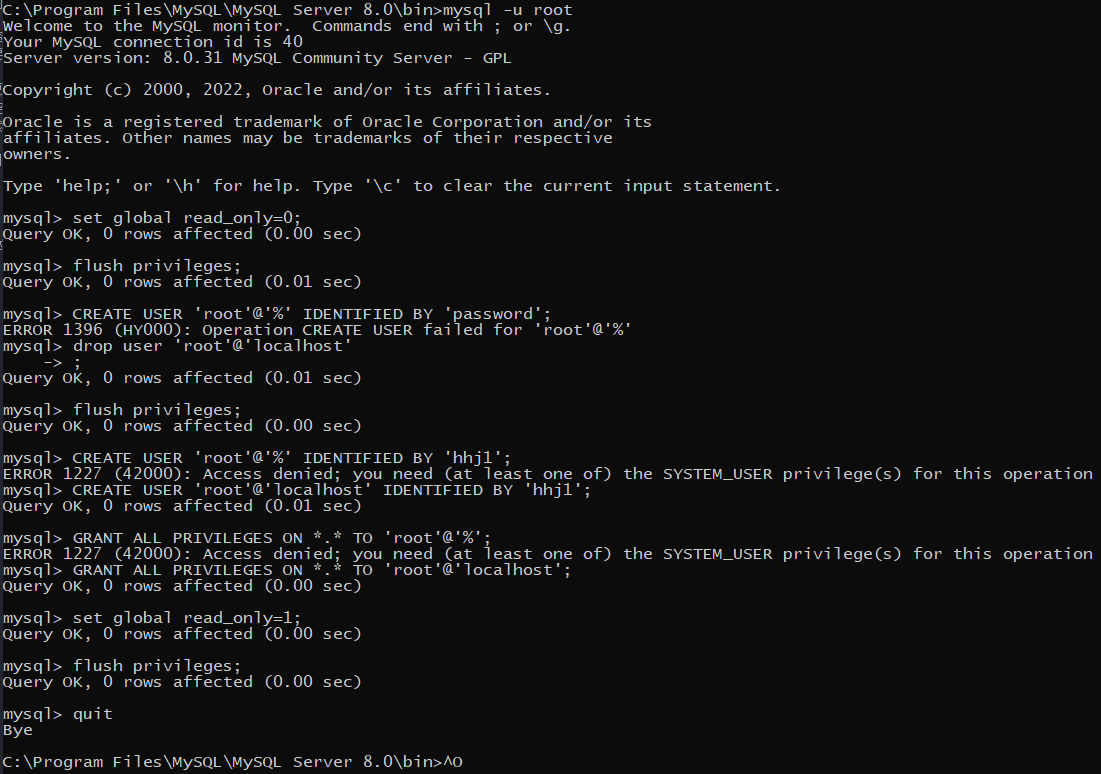
\includegraphics[width=.9\linewidth]{./pic/readme_20230111_162732.png}
% Emacs 27.2 (Org mode 8.2.7c)
\end{document}